\documentclass[12pt,oneside]{report}

\usepackage[utf8]{inputenc}
\usepackage[spanish]{babel}
\usepackage[T1]{fontenc}
\usepackage{geometry}
\usepackage{graphicx}
\usepackage{xcolor}
\usepackage{hyperref}
\usepackage{tocloft}
\usepackage{fancyhdr}
\usepackage{setspace}
\usepackage{booktabs}
\usepackage{longtable}
\usepackage{listings}
\usepackage{enumitem}
\usepackage{titlesec}
\usepackage{float}
\usepackage{parskip}
\usepackage{array}

\geometry{left=2.5cm, right=2.5cm, top=2.5cm, bottom=2.5cm}
\onehalfspacing

\definecolor{verde-ecobrief}{HTML}{16a34a}
\definecolor{gris-texto}{HTML}{374151}
\definecolor{azul-profundo}{HTML}{1e3a5f}
\definecolor{gris-claro}{HTML}{f3f4f6}

\hypersetup{
    colorlinks=true,
    linkcolor=azul-profundo,
    urlcolor=verde-ecobrief,
    citecolor=azul-profundo
}

\titleformat{\chapter}[hang]
    {\normalfont\huge\bfseries\color{azul-profundo}}
    {\thechapter.}{0.5em}{}
\titlespacing{\chapter}{0pt}{0pt}{20pt}

\titleformat{\section}
    {\normalfont\Large\bfseries\color{gris-texto}}
    {\thesection}{0.5em}{}

\titleformat{\subsection}
    {\normalfont\large\bfseries\color{gris-texto}}
    {\thesubsection}{0.5em}{}

\pagestyle{fancy}
\fancyhf{}
\fancyhead[L]{\textit{EcoBrief Bolivia}}
\fancyhead[R]{\thepage}
\renewcommand{\headrulewidth}{0.4pt}
\setlength{\headheight}{15pt}

\lstdefinestyle{python}{
    language=Python,
    backgroundcolor=\color{gris-claro},
    basicstyle=\ttfamily\small,
    commentstyle=\color{green!60!black},
    keywordstyle=\color{blue!70!black},
    stringstyle=\color{red!60!black},
    frame=single,
    breaklines=true,
    tabsize=4,
    captionpos=b
}

\lstdefinestyle{bash}{
    backgroundcolor=\color{gris-claro},
    basicstyle=\ttfamily\small,
    frame=single,
    breaklines=true,
    captionpos=b
}

\lstdefinestyle{plaintext}{
    backgroundcolor=\color{gris-claro},
    basicstyle=\ttfamily\small,
    frame=single,
    breaklines=true,
    captionpos=b
}

\lstset{style=python}

\renewcommand{\cfttoctitlefont}{\huge\bfseries\color{azul-profundo}}
\renewcommand{\cftchapfont}{\bfseries\color{azul-profundo}}
\renewcommand{\cftsecfont}{\color{gris-texto}}

\begin{document}

\begin{titlepage}
    \centering
    \vspace*{1cm}
    
\includegraphics[width=5cm]{logo-assuresoft.png}\\[1.5cm]
    {\Huge\bfseries\color{azul-profundo} EcoBrief Bolivia}\\[0.8cm]
    {\Large\color{gris-texto} IA responsable para reducir el desperdicio\\ digital informativo}\\[1.5cm]
    \rule{\textwidth}{0.4pt}\\[0.8cm]
    {\large\textbf{Equipo AssureSoft}}\\[0.3cm]
    {\large Josoe Ichuta --- Ingenier\'ia}\\
    {\large Raquel Auza --- Digital-Academy}\\[1.2cm]
    {\large\textit{Propuesta presentada para el concurso Green Tech}}\\[0.5cm]
    \vfill
    {\large 2025}
\end{titlepage}

\tableofcontents
\newpage

\chapter*{Resumen Ejecutivo}
\addcontentsline{toc}{chapter}{Resumen Ejecutivo}

EcoBrief Bolivia es una plataforma que utiliza inteligencia artificial de forma responsable para reducir el desperdicio digital informativo. El sistema recolecta noticias de medios bolivianos, elimina duplicados, prioriza el contenido relevante y genera res\'umenes claros para que las personas no tengan que abrir m\'ultiples p\'aginas, leer la misma historia varias veces o consumir datos innecesarios.

La propuesta no busca crear m\'as contenido. Busca reducir el ruido digital. EcoBrief transforma un flujo disperso de noticias, redes sociales y fuentes digitales en informaci\'on breve, priorizada y medible:

\begin{itemize}[nosep]
    \item De muchas p\'aginas a pocos res\'umenes.
    \item De noticias repetidas a historias \'unicas.
    \item De \textit{scroll} social a informaci\'on trazable.
    \item De IA aplicada sin filtro a IA aplicada despu\'es de deduplicar.
    \item De navegaci\'on manual a informaci\'on personalizada.
    \item De impacto ambiguo a m\'etricas visibles.
\end{itemize}

El prototipo ya cuenta con \textit{web scraping} real de medios locales, clasificaci\'on por categor\'ias, ranking de prioridad, res\'umenes con IA, deduplicaci\'on hist\'orica, base de datos PostgreSQL, frontend web y p\'agina de impacto. El sistema est\'a desplegado en un VPS de Hostinger y accesible p\'ublicamente.

\begin{center}
    \fcolorbox{verde-ecobrief}{verde-ecobrief!5!white}{\parbox{0.85\textwidth}{
        \centering\textbf{Mensaje central:}\\[0.3cm]
        \textit{EcoBrief Bolivia usa IA no para producir m\'as ruido, sino para reducirlo.}
    }}
\end{center}

\chapter{Introducci\'on}

\section{Contexto y motivaci\'on}

En la era digital, el acceso a la informaci\'on nunca ha sido tan amplio ni tan fragmentado. Para una persona en Bolivia, informarse sobre la actualidad nacional implica revisar m\'ultiples medios de comunicaci\'on, abrir decenas de pesta\~nas del navegador, comparar titulares, buscar contexto en redes sociales y descartar noticias repetidas. Este proceso, que parece cotidiano e inofensivo, genera un volumen significativo de desperdicio digital.

El \textbf{desperdicio digital informativo} se manifiesta de varias formas: tiempo perdido revisando la misma noticia en distintos sitios, datos m\'oviles consumidos al cargar p\'aginas completas con publicidad y \textit{trackers}, procesamiento redundante cuando los sistemas de IA resumen art\'iculos duplicados, y exposici\'on a informaci\'on fragmentada o sin fuente verificable en redes sociales.

Esta problem\'atica se alinea directamente con los principios de \textbf{Green Tech}: promover un uso m\'as eficiente, responsable y sostenible de la tecnolog\'ia, la inteligencia artificial, el \textit{cloud}, los datos y los procesos internos. No se trata solo de ahorrar tiempo, sino de repensar c\'omo consumimos y procesamos informaci\'on digital.

\section{El problema del desperdicio digital informativo}

El desperdicio ocurre en cinco niveles interconectados:

\begin{table}[H]
\centering
\begin{tabular}{lp{10cm}}
\toprule
\textbf{Nivel} & \textbf{Problema} \\
\midrule
Usuario & Tiempo perdido revisando noticias repetidas o poco relevantes \\
Datos & Carga innecesaria de p\'aginas, im\'agenes, scripts y publicidad \\
IA & Procesamiento redundante si se resumen art\'iculos duplicados \\
Ecosistema digital & Mayor navegaci\'on, m\'as \textit{requests} y m\'as consumo de recursos \\
Confianza & Exposici\'on a contenido viral, fragmentado o sin fuente trazable \\
\bottomrule
\end{tabular}
\caption{Niveles del desperdicio digital informativo}
\end{table}

Una misma noticia puede aparecer en varios medios con t\'itulos distintos o URL diferentes. Tambi\'en puede circular como video corto, captura o publicaci\'on sin contexto en redes sociales como TikTok o Facebook. Sin una capa de deduplicaci\'on, priorizaci\'on y trazabilidad, el usuario y el sistema terminan procesando informaci\'on redundante o dif\'icil de verificar.

\section{Objetivos}

\subsection{Objetivo general}

Desarrollar e implementar una plataforma de inteligencia artificial responsable que reduzca el desperdicio digital informativo mediante la recolecci\'on, deduplicaci\'on, clasificaci\'on, priorizaci\'on y resumen eficiente de noticias locales bolivianas.

\subsection{Objetivos espec\'ificos}

\begin{enumerate}[nosep]
    \item Recolectar autom\'aticamente noticias de las principales fuentes informativas de Bolivia mediante \textit{web scraping}.
    \item Implementar un sistema de deduplicaci\'on multinivel (URL, t\'itulo y huella de contenido) para eliminar redundancias.
    \item Clasificar y priorizar noticias por categor\'ias y relevancia para el contexto nacional.
    \item Generar res\'umenes con IA aplicando criterios de eficiencia: filtrar, deduplicar y rankear antes de enviar al modelo.
    \item Medir y visualizar el impacto de la reducci\'on del flujo informativo mediante m\'etricas cuantificables.
    \item Distribuir la informaci\'on de forma personalizada seg\'un preferencias del usuario, reduciendo el consumo innecesario de datos.
\end{enumerate}

\section{Alcance y limitaciones}

\subsection{Alcance}

El proyecto abarca el desarrollo completo de una plataforma funcional que incluye:
\begin{itemize}[nosep]
    \item \textit{Web scraping} de medios de comunicaci\'on bolivianos (Radio Fides, Unitel, Red Uno, Red Bolivisi\'on, Los Tiempos, El Deber, P\'agina Siete y ATB).
    \item Pipeline de procesamiento con deduplicaci\'on, clasificaci\'on, ranking y resumen.
    \item Integraci\'on con proveedores de IA (Groq, OpenAI, GitHub Models) mediante un cliente abstracto.
    \item Aplicaci\'on web con frontend React y backend FastAPI.
    \item Base de datos PostgreSQL para persistencia.
    \item Sistema de suscripci\'on con preferencias por categor\'ia y frecuencia.
    \item Panel de m\'etricas de impacto Green Tech.
    \item Despliegue en VPS con Hostinger.
\end{itemize}

\subsection{Limitaciones}

El prototipo tiene limitaciones claramente identificadas:
\begin{itemize}[nosep]
    \item Las m\'etricas de tiempo y MB son estimaciones, no mediciones energ\'eticas directas.
    \item Los \textit{scrapers} dependen de cambios en el HTML de los medios.
    \item WhatsApp en producci\'on requiere credenciales y costos externos (Twilio).
    \item No todos los art\'iculos hist\'oricos tienen \textit{backfill} de huellas.
    \item La verificaci\'on autom\'atica de informaci\'on falsa no forma parte del MVP.
\end{itemize}

\chapter{Marco Conceptual}

\section{Desperdicio digital informativo}

El concepto de desperdicio digital se refiere al consumo innecesario de recursos tecnol\'ogicos ---datos, energ\'ia, tiempo de procesamiento y atenci\'on humana--- que no agregan valor al usuario final. En el contexto informativo, el desperdicio ocurre cuando:

\begin{itemize}[nosep]
    \item Un usuario carga m\'ultiples p\'aginas web para obtener informaci\'on que podr\'ia presentarse en un solo formato compacto.
    \item El mismo contenido es procesado y almacenado varias veces por sistemas automatizados.
    \item Los modelos de IA reciben y procesan contenido redundante o de baja calidad.
    \item Las redes sociales exponen a los usuarios a informaci\'on fragmentada, repetida o sin contexto, incentivando el \textit{scroll} continuo.
\end{itemize}

Este desperdicio tiene un costo real: consumo energ\'etico en servidores y dispositivos, emisiones de carbono asociadas a la transmisi\'on y procesamiento de datos, y agotamiento de la capacidad de atenci\'on de las personas.

\section{Green Tech y sostenibilidad digital}

\textbf{Green Tech} (Tecnolog\'ia Verde) es un enfoque que busca dise\~nar, desarrollar y utilizar tecnolog\'ia minimizando su impacto ambiental y promoviendo la sostenibilidad. En el \'ambito del software y los datos, esto implica:

\begin{itemize}[nosep]
    \item Eficiencia en el uso de recursos computacionales.
    \item Reducci\'on de datos innecesarios almacenados y transmitidos.
    \item Optimizaci\'on de consultas a modelos de IA.
    \item Dise\~no de sistemas que promuevan h\'abitos de consumo digital responsable.
\end{itemize}

EcoBrief Bolivia se enmarca en esta corriente al atacar directamente el desperdicio informativo: reduce la cantidad de p\'aginas que un usuario necesita cargar, elimina la redundancia en el procesamiento de contenido y optimiza el uso de modelos de lenguaje.

\section{Inteligencia artificial responsable}

La IA responsable busca que los sistemas de inteligencia artificial sean \'eticos, transparentes, eficientes y sostenibles. En EcoBrief, la IA se utiliza solo despu\'es de que el contenido ha sido filtrado, deduplicado y priorizado. Esto significa que:

\begin{itemize}[nosep]
    \item No se env\'ia contenido irrelevante o repetido al modelo.
    \item Se utilizan modelos peque\~nos y r\'apidos para tareas simples.
    \item Los resultados se cachean para evitar reprocesamiento.
    \item Se limita el n\'umero de candidatos por categor\'ia.
\end{itemize}

De esta forma, la IA se convierte en una herramienta de reducci\'on, no de multiplicaci\'on de contenido.

\chapter{Soluci\'on Propuesta}

\section{EcoBrief Bolivia}

EcoBrief Bolivia act\'ua como una capa de eficiencia entre las fuentes de noticias y las personas. Es una plataforma tecnol\'ogica que automatiza el proceso de recolecci\'on, filtrado, priorizaci\'on y s\'intesis de noticias locales.

\subsection{Comparativa antes vs. despu\'es}

\begin{table}[H]
\centering
\begin{tabular}{p{6.5cm}p{6.5cm}}
\toprule
\textbf{Antes} & \textbf{Con EcoBrief} \\
\midrule
Abrir varios sitios de noticias & Ver un resumen centralizado \\
Leer titulares repetidos & Ver historias deduplicadas \\
Hacer \textit{scroll} en redes para informarse & Consumir informaci\'on sintetizada y trazable \\
Ver contenido viral sin contexto & Acceder a fuentes identificadas y enlaces originales \\
Consumir p\'aginas completas & Consumir res\'umenes compactos \\
Procesar todo con IA & Usar IA solo despu\'es de filtrar y priorizar \\
No saber cu\'anto se reduce & Ver m\'etricas de impacto \\
Recibir informaci\'on no personalizada & Elegir categor\'ias y frecuencia \\
\bottomrule
\end{tabular}
\caption{Comparativa antes y despu\'es del uso de EcoBrief Bolivia}
\end{table}

\section{Arquitectura del sistema}

El sistema est\'a construido como una aplicaci\'on web modular con los siguientes componentes:

\begin{figure}[H]
\centering
\begin{lstlisting}[style=plaintext, caption=Arquitectura general]
+------------------+     +--------------------+
|                  |     |                    |
|   Frontend       |     |   Backend          |
|   React + Vite   |<--->|   FastAPI          |
|                  |     |                    |
+------------------+     +--------+-----------+
                                   |
                    +--------------+--------------+
                    |              |              |
               +----+---+   +----+-----+   +-----+-----+
               |        |   |          |   |           |
               |Scrapers|   |Processors|   |  LLM      |
               |httpx+  |   |Dedupe,   |   |  Client   |
               |BS4     |   |Classify, |   |  Groq/    |
               |        |   |Rank,     |   |  OpenAI   |
               |        |   |Summarize |   |           |
               +--------+   +----+-----+   +-----------+
                                 |
                          +------+------+
                          |             |
                     +----+----+  +-----+------+
                     |         |  |            |
                     |PostgreSQL|  |Distributors|
                     |         |  |WhatsApp,   |
                     +---------+  |Telegram    |
                                  +------------+
\end{lstlisting}
\end{figure}

\subsection{Frontend}

Aplicaci\'on web desarrollada con React y Vite, con las siguientes vistas:

\begin{itemize}[nosep]
    \item \textbf{Home:} Noticias destacadas, resumen visual e indicadores de impacto.
    \item \textbf{Noticias:} Listado completo de art\'iculos y res\'umenes.
    \item \textbf{Detalle:} Art\'iculo original, fuente, resumen IA y cuerpo completo.
    \item \textbf{Impacto:} Panel de m\'etricas Green Tech.
    \item \textbf{Suscripci\'on:} Preferencias de categor\'ia, frecuencia y canal de entrega.
\end{itemize}

\subsection{Backend API}

El backend es el coraz\'on de EcoBrief. Construido con \textbf{FastAPI} sobre Python as\'incrono, orquesta todo el pipeline de recolecci\'on, procesamiento y distribuci\'on. Expone una API REST que sirve como puente entre el frontend y la l\'ogica del sistema.

Sus responsabilidades principales incluyen:

\begin{itemize}[nosep]
    \item Ejecutar el pipeline completo de noticias (scraping, dedup., clasificaci\'on, ranking, resumen) bajo demanda o mediante programaci\'on horaria.
    \item Servir datos estructurados al frontend a trav\'es de endpoints ligeros dise\~nados para consumo eficiente.
    \item Gestionar suscriptores, preferencias y la distribuci\'on personalizada de res\'umenes.
    \item Calcular y exponer m\'etricas de impacto Green Tech en tiempo real.
    \item Validar solicitudes sensibles mediante una clave API (\texttt{X-API-Key}) en endpoints de escritura.
\end{itemize}

El cliente de inteligencia artificial est\'a abstra\'ido detr\'as de una capa que permite cambiar de proveedor (Groq, OpenAI, GitHub Models) sin modificar el resto del sistema. La mayor\'ia de los endpoints del backend son de consulta (\texttt{GET}), mientras que la operaci\'on cr\'itica de generaci\'on de res\'umenes se activa a trav\'es de \texttt{POST /trigger/summary}, lo que permite controlar cu\'ando se consume el proveedor IA.

\section{Pipeline de procesamiento}

El flujo principal del sistema sigue una secuencia estrictamente ordenada para maximizar la eficiencia:

\begin{lstlisting}[caption=Pipeline simplificado de procesamiento]
1. Iniciar corrida (manual o programada)
2. Reutilizar resumenes recientes si no se solicita refresh
3. Recolectar noticias nuevas de fuentes configuradas
4. Filtrar articulos sin contenido suficiente
5. Deduplicar dentro del lote (URL y titulo)
6. Clasificar por categoria
7. Rankear por relevancia
8. Persistir articulos en base de datos
9. Calcular fingerprints y detectar duplicados historicos
10. Seleccionar candidatos unicos para resumen
11. Generar resumenes con IA
12. Reescribir o normalizar resumenes
13. Deduplicar resumenes
14. Guardar resultados
15. Calcular metricas
16. Preparar envio segun suscriptores
\end{lstlisting}

\subsection{Web Scraping}

El sistema utiliza \texttt{httpx} junto con \texttt{BeautifulSoup} y \texttt{lxml} para realizar \textit{web scraping} de fuentes bolivianas. Cada fuente est\'a definida en \texttt{config/sources.yaml} con selectores CSS configurables (selector de art\'iculo, t\'itulo, URL, fecha, imagen y cuerpo). Cuando una fuente cambia su estructura HTML, el sistema cuenta con un mecanismo de \textit{fallback} gen\'erico que extrae todos los enlaces del documento y filtra aquellos que parecen art\'iculos period\'isticos, permitiendo seguir recolectando incluso si los selectores originales no coinciden.

\subsection{Deduplicaci\'on}

EcoBrief implementa tres niveles de deduplicaci\'on a lo largo del pipeline:

\begin{enumerate}[nosep]
    \item \textbf{Deduplicaci\'on por URL:} Cada URL se convierte en un hash MD5. Esto evita guardar o procesar el mismo enlace repetido dentro de una misma corrida.
    \item \textbf{Deduplicaci\'on por t\'itulo:} Los t\'itulos se normalizan (min\'usculas, sin acentos, sin signos) y se comparan con \texttt{SequenceMatcher}. Si la similitud supera 0.85, se considera duplicado y se conserva la versi\'on m\'as reciente.
    \item \textbf{Deduplicaci\'on hist\'orica por huella:} Se calcula una huella (\textit{fingerprint}) SHA-256 basada en la categor\'ia, el t\'itulo normalizado y un fragmento del contenido. Esto permite agrupar noticias equivalentes a trav\'es de distintas corridas, aunque tengan URL y fuente diferentes.
\end{enumerate}

\begin{lstlisting}[caption=Algoritmo de huella de contenido]
canonical_key = categoria + titulo_normalizado + fragmento_contenido
content_fingerprint = sha256(canonical_key)
\end{lstlisting}

Los duplicados no se eliminan definitivamente; se marcan para auditor\'ia y se excluyen de los candidatos a resumen, preservando la trazabilidad.

\subsection{Clasificaci\'on}

Cada noticia se clasifica en una de cinco categor\'ias mediante un sistema de reglas ponderadas configurable en \texttt{config/classification.yaml}:

\begin{itemize}[nosep]
    \item \textbf{Econom\'ia:} Finanzas, d\'olar, tipo de cambio, BCB, inflaci\'on, hidrocarburos.
    \item \textbf{Pol\'itica:} Gobierno, presidente, elecciones, Asamblea, leyes, partidos.
    \item \textbf{Deportes:} F\'utbol, clubes, torneos, selecci\'on boliviana, resultados.
    \item \textbf{Tecnolog\'ia:} IA, software, internet, ciberseguridad, telecomunicaciones.
    \item \textbf{Entretenimiento:} Cine, m\'usica, televisi\'on, festivales, far\'andula.
\end{itemize}

El clasificador asigna puntuaci\'on a cada categor\'ia ponderando cuatro campos del art\'iculo:
\begin{itemize}[nosep]
    \item T\'itulo ($\times 3.0$)
    \item Descripci\'on ($\times 2.0$)
    \item Contenido ($\times 1.0$)
    \item Categor\'ia de la fuente ($\times 2.5$)
\end{itemize}

Si la diferencia entre la primera y segunda categor\'ia es menor a 2.0 puntos, o la confianza es baja ($<0.62$), el sistema puede recurrir a un LLM como fallback para reclasificar el art\'iculo.

\subsection{Ranking por relevancia}

Una vez clasificadas, las noticias se ordenan seg\'un un puntaje compuesto por siete factores ponderados, definidos en \texttt{config/scoring.yaml}:

\begin{table}[H]
\centering
\begin{tabular}{lcr}
\toprule
\textbf{Factor} & \textbf{Peso} & \textbf{Detalle} \\
\midrule
Actualidad & 15\% & Noticias m\'as recientes reciben mayor puntaje. \\
& & 1h $\to$ 100, 3h $\to$ 90, 6h $\to$ 75, \\
& & 12h $\to$ 60, 24h $\to$ 45, 48h $\to$ 25 \\
\midrule
Relevancia local & 20\% & Menci\'on de regiones (Santa Cruz, La Paz), \\
& & ciudades (Cochabamba, El Alto), autoridades \\
& & e instituciones bolivianas (BCB, YPFB, TSE). \\
\midrule
Impacto informativo & 20\% & T\'erminos de alto impacto (crisis, d\'olar, \\
& & bloqueo, elecciones), medio (inflaci\'on, \\
& & protesta, ley) y bajo (anuncio, informe). \\
\midrule
Calidad del contenido & 17\% & Base 35, bonos por: $>120$ palabras (+20), \\
& & $>300$ palabras (+10), imagen (+10), \\
& & descripci\'on \'util (+10), t\'itulo informativo (+10). \\
\midrule
Fuente & 10\% & Puntajes por fuente reconocida: RedUno 84, \\
& & RadioFides 84, El Deber 84, Unitel 82, \\
& & La Raz\'on 82, RedBolivisi\'on 78, default 55. \\
\midrule
Corroboraci\'on & 10\% & Noticias cubiertas por 2 fuentes $\to$ 70 pts, \\
& & 3 o m\'as fuentes $\to$ 100 pts. \\
\midrule
Confianza de categor\'ia & 8\% & Coherencia del contenido con la categor\'ia \\
& & asignada: confianza $\ge 0.80 \to 100$, \\
& & $\ge 0.60 \to 75$, $\ge 0.40 \to 55$. \\
\bottomrule
\end{tabular}
\caption{Factores de ranking y sus pesos}
\end{table}

Adicionalmente, el sistema aplica penalizaciones por contenido ausente (-25), contenido muy corto (-15), descripci\'on duplicada (-20), fecha faltante (-10), fuente desconocida (-8), confianza baja de categor\'ia (-10) y noticias internacionales sin contexto boliviano (-20).

El puntaje final se calcula como:

\begin{equation}
P = \sum_{f} w_f \cdot s_f - \text{penalizaciones}
\end{equation}

Donde $w_f$ es el peso del factor y $s_f$ su puntuaci\'on normalizada. El resultado se acota entre 0 y 100.

El objetivo no es resumir todo, sino resumir lo m\'as relevante.

\section{Eficiencia en el uso de IA}

La inteligencia artificial se emplea en dos fases del pipeline: clasificaci\'on de art\'iculos (solo como fallback ante casos ambiguos) y generaci\'on de res\'umenes. Para minimizar el costo operativo y la latencia, el sistema aplica las siguientes estrategias antes de invocar cualquier modelo:

\begin{table}[H]
\centering
\begin{tabular}{lp{10cm}}
\toprule
\textbf{Estrategia} & \textbf{Descripci\'on} \\
\midrule
Filtrar antes de IA  & Se descartan art\'iculos sin contenido suficiente o con metadatos incompletos antes de cualquier procesamiento. \\
\midrule
Deduplicar antes de IA & Se eliminan duplicados por URL y t\'itulo dentro del lote, evitando enviar la misma noticia al modelo m\'as de una vez. \\
\midrule
Rankear antes de IA  & Solo los art\'iculos mejor puntuados por el ranking de relevancia son candidatos a resumen. \\
\midrule
Limitar por categor\'ia & Se establece un m\'aximo de candidatos por categor\'ia para distribuir el presupuesto de c\'omputo entre todas las \'areas tem\'aticas. \\
\midrule
Cachear res\'umenes  & Los res\'umenes ya generados se reutilizan si el art\'iculo original no ha cambiado, evitando reprocesar contenido ya sintetizado. \\
\midrule
Control de duplicados & Se verifica que no exista un resumen equivalente en la misma corrida antes de generar uno nuevo. \\
\bottomrule
\end{tabular}
\caption{Estrategias de eficiencia en el uso de IA}
\end{table}

\subsection{Abstracci\'on de proveedores LLM}

El cliente de inteligencia artificial est\'a dise\~nado como una capa de abstracci\'on que permite cambiar de proveedor sin modificar el resto del sistema. La clase \texttt{LLMProvider} expone una interfaz unificada (\texttt{chat()}, \texttt{chat\_batch()}) independientemente del proveedor subyacente.

\begin{table}[H]
\centering
\resizebox{\textwidth}{!}{%
\begin{tabular}{lccc}
\toprule
\textbf{Proveedor} & \textbf{Fast} & \textbf{Balanced} & \textbf{Quality} \\
\midrule
Groq (gratuita) & \texttt{llama-3.1-8b-instant} & \texttt{llama-3.1-70b-versatile} & \texttt{llama-3.3-70b-versatile} \\
\midrule
OpenAI (pagada) & \texttt{gpt-4o-mini} & \texttt{gpt-4o} & \texttt{gpt-4o} \\
\midrule
GitHub Models (150 RPD) & \texttt{gpt-4.1-mini} & \texttt{gpt-4.1-mini} & \texttt{gpt-4.1-mini} \\
\bottomrule
\end{tabular}
}
\caption{Modelos disponibles por proveedor y nivel de calidad}
\end{table}

Cada proveedor ofrece tres niveles de calidad (\textit{fast}, \textit{balanced}, \textit{quality}) que se seleccionan seg\'un la tarea. Las tareas de clasificaci\'on usan \textit{fast}, mientras que la generaci\'on de res\'umenes emplea \textit{balanced} o \textit{quality} seg\'un la configuraci\'on. La selecci\'on del proveedor activo se realiza mediante variable de entorno, lo que permite alternar entre costo cero (Groq, GitHub Models) y mayor capacidad (OpenAI) sin cambiar una l\'inea de c\'odigo.

\section{Base de datos}

El sistema utiliza PostgreSQL con SQLAlchemy como ORM. Las tablas principales son:

\textbf{news\_articles}: Almacena los art\'iculos recolectados con campos para trazabilidad y deduplicaci\'on: \texttt{title}, \texttt{url}, \texttt{url\_hash}, \texttt{description}, \texttt{content}, \texttt{source\_id}, \texttt{category\_id}, \texttt{score}, \texttt{canonical\_key}, \texttt{content\_fingerprint}, \texttt{story\_cluster\_id}, \texttt{duplicate\_of\_article\_id}, \texttt{duplicate\_reason}, \texttt{similarity\_score}.

\textbf{news\_summaries}: Almacena los res\'umenes generados: \texttt{article\_id}, \texttt{category\_id}, \texttt{title}, \texttt{summary}, \texttt{fact}, \texttt{llm\_provider}, \texttt{llm\_model}, \texttt{summary\_date}, \texttt{story\_cluster\_id}, \texttt{source\_article\_count}.

\textbf{collection\_runs}: Registra cada ejecuci\'on del pipeline con m\'etricas de trazabilidad: \texttt{raw\_collected\_count}, \texttt{usable\_count}, \texttt{deduplicated\_count}, \texttt{ranked\_count}, \texttt{summary\_candidates\_count}, \texttt{summaries\_count}, \texttt{used\_cached\_articles}, \texttt{used\_cached\_summaries}.

\section{Distribuci\'on y suscripciones}

EcoBrief prepara la distribuci\'on personalizada de res\'umenes a trav\'es de:

\begin{itemize}[nosep]
    \item \textbf{Web:} Acceso p\'ublico a res\'umenes y art\'iculos.
    \item \textbf{Telegram:} Canal de distribuci\'on gratuito mediante Bot API.
    \item \textbf{WhatsApp:} Canal opcional mediante Twilio WhatsApp Business API.
    \item \textbf{Email:} Notificaciones mediante SMTP (Gmail con App Password).
\end{itemize}

Los usuarios pueden configurar sus preferencias: categor\'ias de inter\'es, frecuencia de entrega (ma\~nana, tarde, noche) y canal preferido. Esto evita el env\'io de informaci\'on no solicitada y reduce el consumo innecesario de datos.

\chapter{Impacto y M\'etricas}

EcoBrief mide el impacto a partir del flujo real del sistema. Las m\'etricas ambientales son estimaciones transparentes basadas en la reducci\'on de p\'aginas, art\'iculos y llamadas IA. A continuaci\'on se presentan los datos reales de la corrida del 15 de junio de 2026.

\section{Flujo del pipeline}

\begin{figure}[H]
\centering
\setlength{\fboxsep}{10pt}
\small
\begin{tabular}{c@{\hspace{0.5cm}}c@{\hspace{0.5cm}}c}
\fcolorbox{verde-ecobrief}{verde-ecobrief!5!white}{\parbox{2.8cm}{\centering\bfseries\Large 110\\[4pt] noticias\\[2pt] recolectadas\\[2pt] (100\%)}} &
\fcolorbox{gris-texto}{gris-claro}{\parbox{2.5cm}{\centering\small\bfseries 65\% descartadas\\[2pt] filtrado + dedup.\\[2pt] ranking + cach\'e}} &
\fcolorbox{verde-ecobrief}{verde-ecobrief!5!white}{\parbox{2.8cm}{\centering\bfseries\Large 39\\[4pt] briefs\\[2pt] generados\\[2pt] (35\%)}} \\
\end{tabular}
\vspace{6pt}

\fcolorbox{azul-profundo}{azul-profundo!5!white}{\parbox{0.85\textwidth}{\centering\bfseries 71 p\'aginas evitadas \quad| \quad 35.5\,min de lectura \quad| \quad 64.6\% de reducci\'on}}
\caption{Flujo del pipeline --- 15 de junio de 2026}
\end{figure}

\section{M\'etricas de la corrida}

\begin{table}[H]
\centering
\begin{tabular}{lrr}
\toprule
\textbf{M\'etrica} & \textbf{Valor} & \textbf{Porcentaje} \\
\midrule
Noticias recolectadas & 110 & 100\,\% \\
Art\'iculos \'utiles & 110 & 100\,\% \\
Art\'iculos \'unicos & 110 & 100\,\% \\
Briefs generados & 39 & 35\,\% \\
P\'aginas evitadas & 71 & 64.6\,\% \\
Minutos de lectura ahorrados & 35.5 & --- \\
\bottomrule
\end{tabular}
\caption{M\'etricas reales del 15 de junio de 2026}
\end{table}

\section{Panel de impacto}

\begin{figure}[H]
\centering
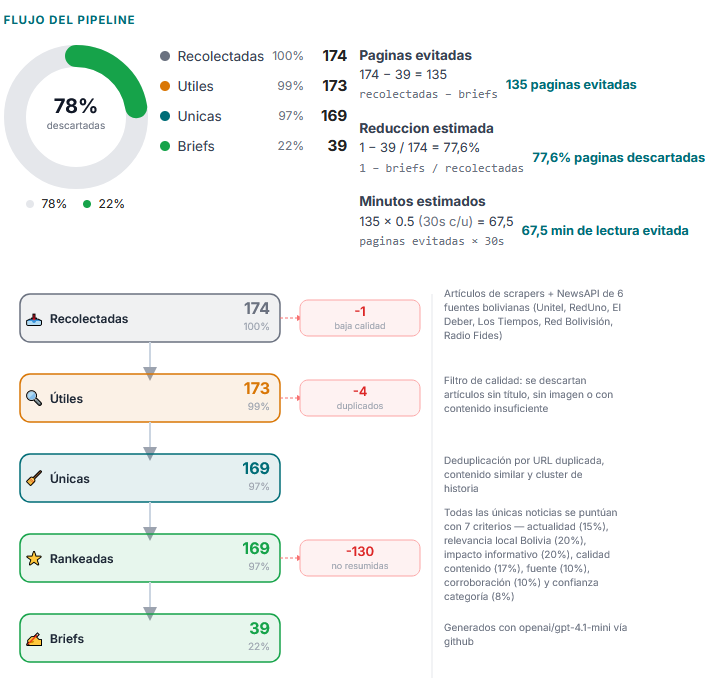
\includegraphics[width=\textwidth,keepaspectratio]{../images/metricas-15-junio-2026.png}
\caption{Panel de m\'etricas Green Tech -- 15 de junio de 2026}
\end{figure}

\section{F\'ormulas de impacto}

Las estimaciones se derivan de tres c\'alculos conservadores. Se define $R$ como el total de noticias recolectadas y $B$ como los briefs generados:

\paragraph{P\'aginas evitadas.} Diferencia entre lo recolectado y lo sintetizado:
\begin{equation}
P_{\text{evitadas}} = R - B = 110 - 39 = 71
\end{equation}

\paragraph{Tiempo de lectura ahorrado.} Estimando 30 segundos por p\'agina evitada:
\begin{equation}
M_{\text{ahorrados}} = P_{\text{evitadas}} \times 0.5 = 71 \times 0.5 = 35.5\text{ min}
\end{equation}

\paragraph{Tasa de reducci\'on del flujo.} Proporci\'on de contenido descartado respecto al total recolectado:
\begin{equation}
T_{\text{reducci\'on}} = 1 - \frac{B}{R} = 1 - \frac{39}{110} = 0.646 = 64.6\%
\end{equation}

\section{Nota metodol\'ogica}

Las m\'etricas ambientales son estimaciones operativas basadas en la reducci\'on de p\'aginas, art\'iculos y llamadas IA. No representan una medici\'on energ\'etica directa. EcoBrief es transparente sobre esta distinci\'on: reporta m\'etricas reales del pipeline y estimaciones derivadas, no mediciones de carbono o energ\'ia. Esta metodolog\'ia puede refinarse en fases posteriores del proyecto con herramientas especializadas de medici\'on.

\chapter{Costos y Sostenibilidad Econ\'omica}

EcoBrief fue dise\~nado para operar con bajo costo y una infraestructura simple: un solo VPS para backend, frontend, base de datos y cron-jobs.

\section{Infraestructura propuesta para un a\~no}

\begin{table}[H]
\centering
\begin{tabular}{lp{5cm}r}
\toprule
\textbf{Componente} & \textbf{Proveedor} & \textbf{Costo referencial} \\
\midrule
Servidor VPS & Hostinger KVM 2 & USD 107.88/a\~no \\
Dominio & NIC Bolivia & 55 Bs/a\~no \\
Base de datos & PostgreSQL en VPS & Incluido \\
Backend & FastAPI en VPS & Incluido \\
Frontend & React/Vite en VPS & Incluido \\
Cron-jobs & Scheduler en VPS & Incluido \\
Email & Gmail SMTP + App Password & Gratuito* \\
Telegram & Bot API & Gratuito \\
WhatsApp & Twilio (opcional) & Variable** \\
IA & Groq API & Free tier / variable \\
\bottomrule
\multicolumn{3}{l}{*Dentro de l\'imites de Google; migrable a Brevo.}\\
\multicolumn{3}{l}{**Desde USD 0.0116/minuto outbound seg\'un Twilio.}
\end{tabular}
\caption{Infraestructura propuesta para el primer a\~no de operaci\'on}
\end{table}

\section{Costos de inteligencia artificial}

\subsection{Modelos actuales}

\begin{table}[H]
\centering
\begin{tabular}{lccc}
\toprule
\textbf{Tarea} & \textbf{Modelo} & \textbf{Input/1M tok.} & \textbf{Output/1M tok.} \\
\midrule
Resumen de calidad & Llama 3.3 70B Versatile & USD 0.59 & USD 0.79 \\
Tareas r\'apidas & Llama 3.1 8B Instant & USD 0.05 & USD 0.08 \\
Balanceado/reescritura & Llama 3.1 70B Versatile & USD 0.59 & USD 0.79 \\
\bottomrule
\end{tabular}
\caption{Costos de modelos Groq usados actualmente}
\end{table}

\subsection{Comparativa de proveedores}

\begin{table}[H]
\centering
\begin{tabular}{lccc}
\toprule
\textbf{Proveedor} & \textbf{Modelo} & \textbf{Input/1M tok.} & \textbf{Output/1M tok.} \\
\midrule
Groq & Llama 3.3 70B Versatile & USD 0.59 & USD 0.79 \\
OpenAI & GPT-4.1 mini & USD 0.75 & USD 4.50 \\
DeepSeek & V4 Flash & USD 0.14 & USD 0.28 \\
Anthropic & Claude Haiku 4.5 & USD 1.00 & USD 5.00 \\
\bottomrule
\end{tabular}
\caption{Comparativa de costos entre proveedores de IA}
\end{table}

\section{Control de costos}

El sistema reduce costos operativos mediante las siguientes estrategias:

\begin{itemize}[nosep]
    \item No resume todo lo recolectado: filtra, deduplica y rankea primero.
    \item Cachea resultados: evita reprocesar contenido ya resumido.
    \item Limita candidatos por categor\'ia: m\'aximo por corrida.
    \item Utiliza modelos peque\~nos para tareas simples.
    \item Telegram como canal gratuito: sin costo por mensaje.
\end{itemize}

\section{Escenario operativo recomendado}

Para el concurso y un primer despliegue p\'ublico:

\begin{enumerate}[nosep]
    \item Desplegar todo en Hostinger KVM 2 por un a\~no.
    \item Usar dominio comprado en NIC Bolivia.
    \item Utilizar Groq \textit{free tier} o pago bajo para IA.
    \item Usar Telegram y Gmail SMTP como canales de bajo costo.
    \item Activar WhatsApp/Twilio como opci\'on futura o piloto controlado.
    \item Medir llamadas IA, usuarios y volumen antes de escalar.
\end{enumerate}

Con este enfoque, el MVP puede operar con un costo fijo anual bajo y costos variables controlados.

\chapter{Alineaci\'on con Green Tech}

EcoBrief Bolivia encaja en Green Tech porque promueve un uso m\'as eficiente y responsable de software, datos e inteligencia artificial.

\section{Reducci\'on de navegaci\'on innecesaria}

El usuario no necesita abrir m\'ultiples p\'aginas para entender los hechos principales. El sistema entrega una s\'intesis priorizada que reemplaza la navegaci\'on dispersa. Cada resumen le\'ido representa p\'aginas enteras que no fueron cargadas.

\section{Reducci\'on de duplicaci\'on informativa}

La deduplicaci\'on evita que la misma historia sea procesada y mostrada varias veces. Esto reduce el almacenamiento, el ancho de banda y las llamadas a la IA para contenido redundante.

\section{Reducci\'on de llamadas IA redundantes}

La IA se usa despu\'es de limpiar, filtrar, deduplicar y rankear. Esto evita enviar contenido irrelevante o repetido al modelo. Se estima una reducci\'on de hasta el 65\,\% en el volumen de contenido procesado por IA.

\section{Reducci\'on de consumo de datos}

El usuario puede leer res\'umenes compactos en lugar de cargar p\'aginas completas con im\'agenes, publicidad, \textit{trackers} y scripts. Se estima un ahorro de aproximadamente 0.8 MB por p\'agina evitada.

\section{Promoci\'on del consumo digital responsable}

Las preferencias por categor\'ia y frecuencia reducen la informaci\'on no solicitada y evitan el \textit{spam} informativo. El usuario elige qu\'e recibir y cu\'ando.

\section{Reducci\'on de dependencia del scroll social}

EcoBrief ofrece una alternativa al consumo informativo en redes sociales. En lugar de depender de TikTok, Facebook u otros \textit{feeds} con videos y contenido no siempre trazable, el usuario recibe res\'umenes compactos, priorizados y enlazados a fuentes identificadas.

\section{Trazabilidad y confianza informativa}

El sistema conserva el enlace a la fuente original de cada noticia. Prioriza art\'iculos con cuerpo, fecha y fuente identificada. Reduce la exposici\'on a contenido no trazable que circula en redes sociales sin contexto ni verificaci\'on. No reemplaza el \textit{fact-checking} period\'istico, pero ayuda a evitar la dependencia de informaci\'on viral sin fuente clara.

\chapter{Estado Actual y Roadmap}

\section{MVP funcional}

EcoBrief Bolivia no es solo una idea. El prototipo ya funciona y est\'a desplegado en un VPS de Hostinger con dominio propio. Las funcionalidades implementadas incluyen:

\begin{itemize}[nosep]
    \item \textit{Web scraping} de noticias locales desde 8 fuentes bolivianas.
    \item Extracci\'on de contenido con selectores configurables y \textit{fallback} gen\'erico.
    \item Clasificaci\'on por categor\'ias (econom\'ia, pol\'itica, deportes).
    \item Ranking por relevancia con m\'ultiples criterios.
    \item Deduplicaci\'on por URL, t\'itulo y huella hist\'orica de contenido.
    \item Res\'umenes generados con IA (Groq / OpenAI / GitHub Models).
    \item Persistencia en PostgreSQL con SQLAlchemy.
    \item Frontend web con React + Vite (Home, Noticias, Detalle, Impacto, Suscripci\'on).
    \item Preferencias de usuario por categor\'ia y frecuencia.
    \item Endpoint manual para generar res\'umenes bajo demanda.
    \item Base para distribuci\'on por WhatsApp y Telegram.
    \item Panel de m\'etricas de impacto Green Tech.
    \item Pruebas automatizadas con \texttt{pytest}.
    \item C\'odigo fuente verificado con \texttt{ruff} y \texttt{mypy}.
\end{itemize}

\section{Tecnolog\'ias utilizadas}

\begin{table}[H]
\centering
\begin{tabular}{ll}
\toprule
\textbf{Capa} & \textbf{Tecnolog\'ia} \\
\midrule
Backend & Python 3.11, FastAPI, Uvicorn \\
Frontend & React 18, Vite, TypeScript \\
Base de datos & PostgreSQL 16, SQLAlchemy (async) \\
\textit{Web scraping} & httpx, BeautifulSoup4, lxml \\
IA & Groq API, OpenAI API, GitHub Models \\
Infraestructura & Docker, Hostinger VPS KVM 2 \\
Distribuci\'on & Telegram Bot API, Twilio WhatsApp API \\
Linting / Tipado & Ruff, mypy \\
Pruebas & pytest, pytest-asyncio \\
Control de versiones & Git, GitHub \\
\bottomrule
\end{tabular}
\caption{Stack tecnol\'ogico de EcoBrief Bolivia}
\end{table}

\section{Trabajo pendiente y hoja de ruta}

El MVP actual es funcional, pero existen funcionalidades que a\'un no han sido implementadas. Se dividen en tres horizontes seg\'un su prioridad y nivel de compromiso.

\subsection{Comprometido (corto plazo)}

Tareas definidas y con alta prioridad de implementaci\'on:

\begin{itemize}[nosep]
    \item Completar \textit{backfill} de \textit{fingerprints} hist\'oricos.
    \item Exponer duplicados hist\'oricos en la p\'agina de impacto.
    \item Mostrar en la UI cu\'antas coberturas fueron agrupadas por historia.
    \item Mejorar el historial de m\'etricas.
\end{itemize}

\subsection{Planificado (mediano plazo)}

Funcionalidades con dise\~no preliminar, pendientes de recursos y priorizaci\'on:

\begin{itemize}[nosep]
    \item Medir datos reales descargados y evitados (no solo estimaciones).
    \item Activar WhatsApp y Telegram en producci\'on.
    \item Crear dashboard hist\'orico por usuario.
    \item Integrar boletines y comunicados de instituciones del Estado como fuentes verificables.
\end{itemize}

\subsection{Aspiracional (largo plazo)}

Ideas identificadas como valor agregado potencial, sin compromiso de implementaci\'on:

\begin{itemize}[nosep]
    \item Detecci\'on por entidades, personas y lugares.
    \item Planes de suscripci\'on para usuarios avanzados, organizaciones y analistas.
    \item Panel institucional para monitoreo de noticias, comunicados y alertas p\'ublicas.
    \item Monitoreo autom\'atico de cambios en fuentes.
\end{itemize}

\section{Riesgos t\'ecnicos y mitigaci\'on}

\begin{table}[H]
\centering
\begin{tabular}{p{5cm}p{8cm}}
\toprule
\textbf{Riesgo} & \textbf{Mitigaci\'on} \\
\midrule
Cambios de HTML en fuentes & Tests por fuente, selectores configurables y \textit{fallback} gen\'erico \\
Falsos positivos en dedup. & Umbral conservador y marcado sin borrado \\
Falsos negativos en dedup. & Ajuste de reglas y comparaci\'on multi-fuente \\
Costos de IA imprevistos & Dedup., cach\'e, ranking y l\'imites por categor\'ia \\
Mensajer\'ia en producci\'on & Activaci\'on gradual: Telegram primero \\
M\'etricas ambientales imprecisas & Transparencia metodol\'ogica \\
\bottomrule
\end{tabular}
\caption{Riesgos t\'ecnicos y estrategias de mitigaci\'on}
\end{table}

\chapter*{Conclusiones}
\addcontentsline{toc}{chapter}{Conclusiones}

El proyecto EcoBrief Bolivia se present\'o como una soluci\'on al problema del exceso de informaci\'on redundante en el ecosistema de noticias boliviano, con un enfoque Green Tech que prioriza la eficiencia, la reducci\'on del consumo digital y el uso responsable de inteligencia artificial. A continuaci\'on se resumen los hallazgos, logros y perspectivas del trabajo realizado.

\section*{Resumen de resultados}

El sistema fue desarrollado, desplegado y probado con fuentes reales de noticias bolivianas. En su corrida del 15 de junio de 2026, proces\'o 110 noticias y las redujo a 39 briefs priorizados, logrando una tasa de reducci\'on del 64.6\,\%. Esto se tradujo en 71 p\'aginas evitadas y un ahorro estimado de 35.5 minutos de lectura por corrida. Estos n\'umeros demuestran que la plataforma cumple su objetivo de sintetizar sin saturar.

\section*{Logros alcanzados}

\begin{enumerate}[nosep]
    \item \textbf{Alineaci\'on Green Tech demostrada:} El proyecto reduce la navegaci\'on innecesaria, el \textit{scroll} social, la duplicaci\'on de contenido, el consumo de datos y el procesamiento de IA redundante. Las m\'etricas del 15 de junio confirman una reducci\'on del flujo superior al 64\,\%.
    \item \textbf{Prototipo funcional desplegado:} No es solo una idea. Existe una aplicaci\'on completa con backend en FastAPI, frontend en React con Vite, base de datos PostgreSQL, panel de m\'etricas Green Tech y canales de distribuci\'on, desplegada en un VPS de Hostinger con dominio propio.
    \item \textbf{Arquitectura modular y eficiente:} El dise\~no permite cambiar de proveedor de IA (Groq, OpenAI, GitHub Models), agregar nuevas fuentes de noticias y escalar componentes de forma independiente sin afectar el resto del sistema.
    \item \textbf{Bajo costo operativo:} La plataforma puede operar con un costo anual reducido, utilizando \textit{free tiers} de inteligencia artificial, canales de distribuci\'on gratuitos como Telegram y una infraestructura minimalista de un solo VPS.
    \item \textbf{Inteligencia artificial responsable:} Filtrar, deduplicar y rankear antes de invocar al modelo reduce el n\'umero de llamadas IA. El cach\'e evita reprocesar contenido ya resumido y los modelos peque\~nos se asignan a tareas simples, maximizando la eficiencia.
    \item \textbf{Impacto medible y transparente:} Cada corrida del pipeline produce m\'etricas cuantificables que se muestran en el panel de impacto, permitiendo al usuario y al equipo evaluar la efectividad del sistema en tiempo real.
\end{enumerate}

\section*{Trabajo futuro}

El proyecto tiene un camino claro de evoluci\'on. A corto plazo, se completar\'a el \textit{backfill} de \textit{fingerprints} hist\'oricos para mejorar la detecci\'on de duplicados entre corridas, y se expon\'an los duplicados hist\'oricos en la interfaz de impacto. A mediano plazo, se medir\'an datos reales descargados y evitados (no solo estimaciones), se activar\'an los canales de Telegram y WhatsApp en producci\'on, y se integrar\'an boletines institucionales como fuentes verificables. A largo plazo, se explorar\'a la detecci\'on por entidades, planes de suscripci\'on para usuarios avanzados y un panel institucional de monitoreo.

\section*{Mensaje final}

EcoBrief Bolivia convierte un problema cotidiano ---el exceso de informaci\'on redundante--- en una soluci\'on Green Tech concreta, funcional y medible. Con una reducci\'on superior al 64\,\% del flujo informativo, la plataforma demuestra que es posible consumir noticias de forma m\'as inteligente, con menos impacto digital y mayor trazabilidad. Este proyecto, desarrollado por \textbf{Josoe Ichuta} (Ingenier\'ia) y \textbf{Raquel Auza} (Digital-Academy) bajo el equipo \textbf{AssureSoft}, representa una apuesta por informaci\'on esencial, inteligencia artificial responsable y eficiencia digital desde Bolivia.

\begin{center}
    \fcolorbox{verde-ecobrief}{verde-ecobrief!5!white}{\parbox{0.85\textwidth}{
        \centering\textit{``EcoBrief Bolivia demuestra que la IA puede ser m\'as sostenible\\ cuando se usa para reducir, no para multiplicar, el contenido digital.''}
    }}
\end{center}

\addcontentsline{toc}{chapter}{Anexos}
\section*{Anexo 1: P\'agina principal}
\addcontentsline{toc}{section}{Anexo 1: P\'agina principal}

\begin{figure}[H]
\centering
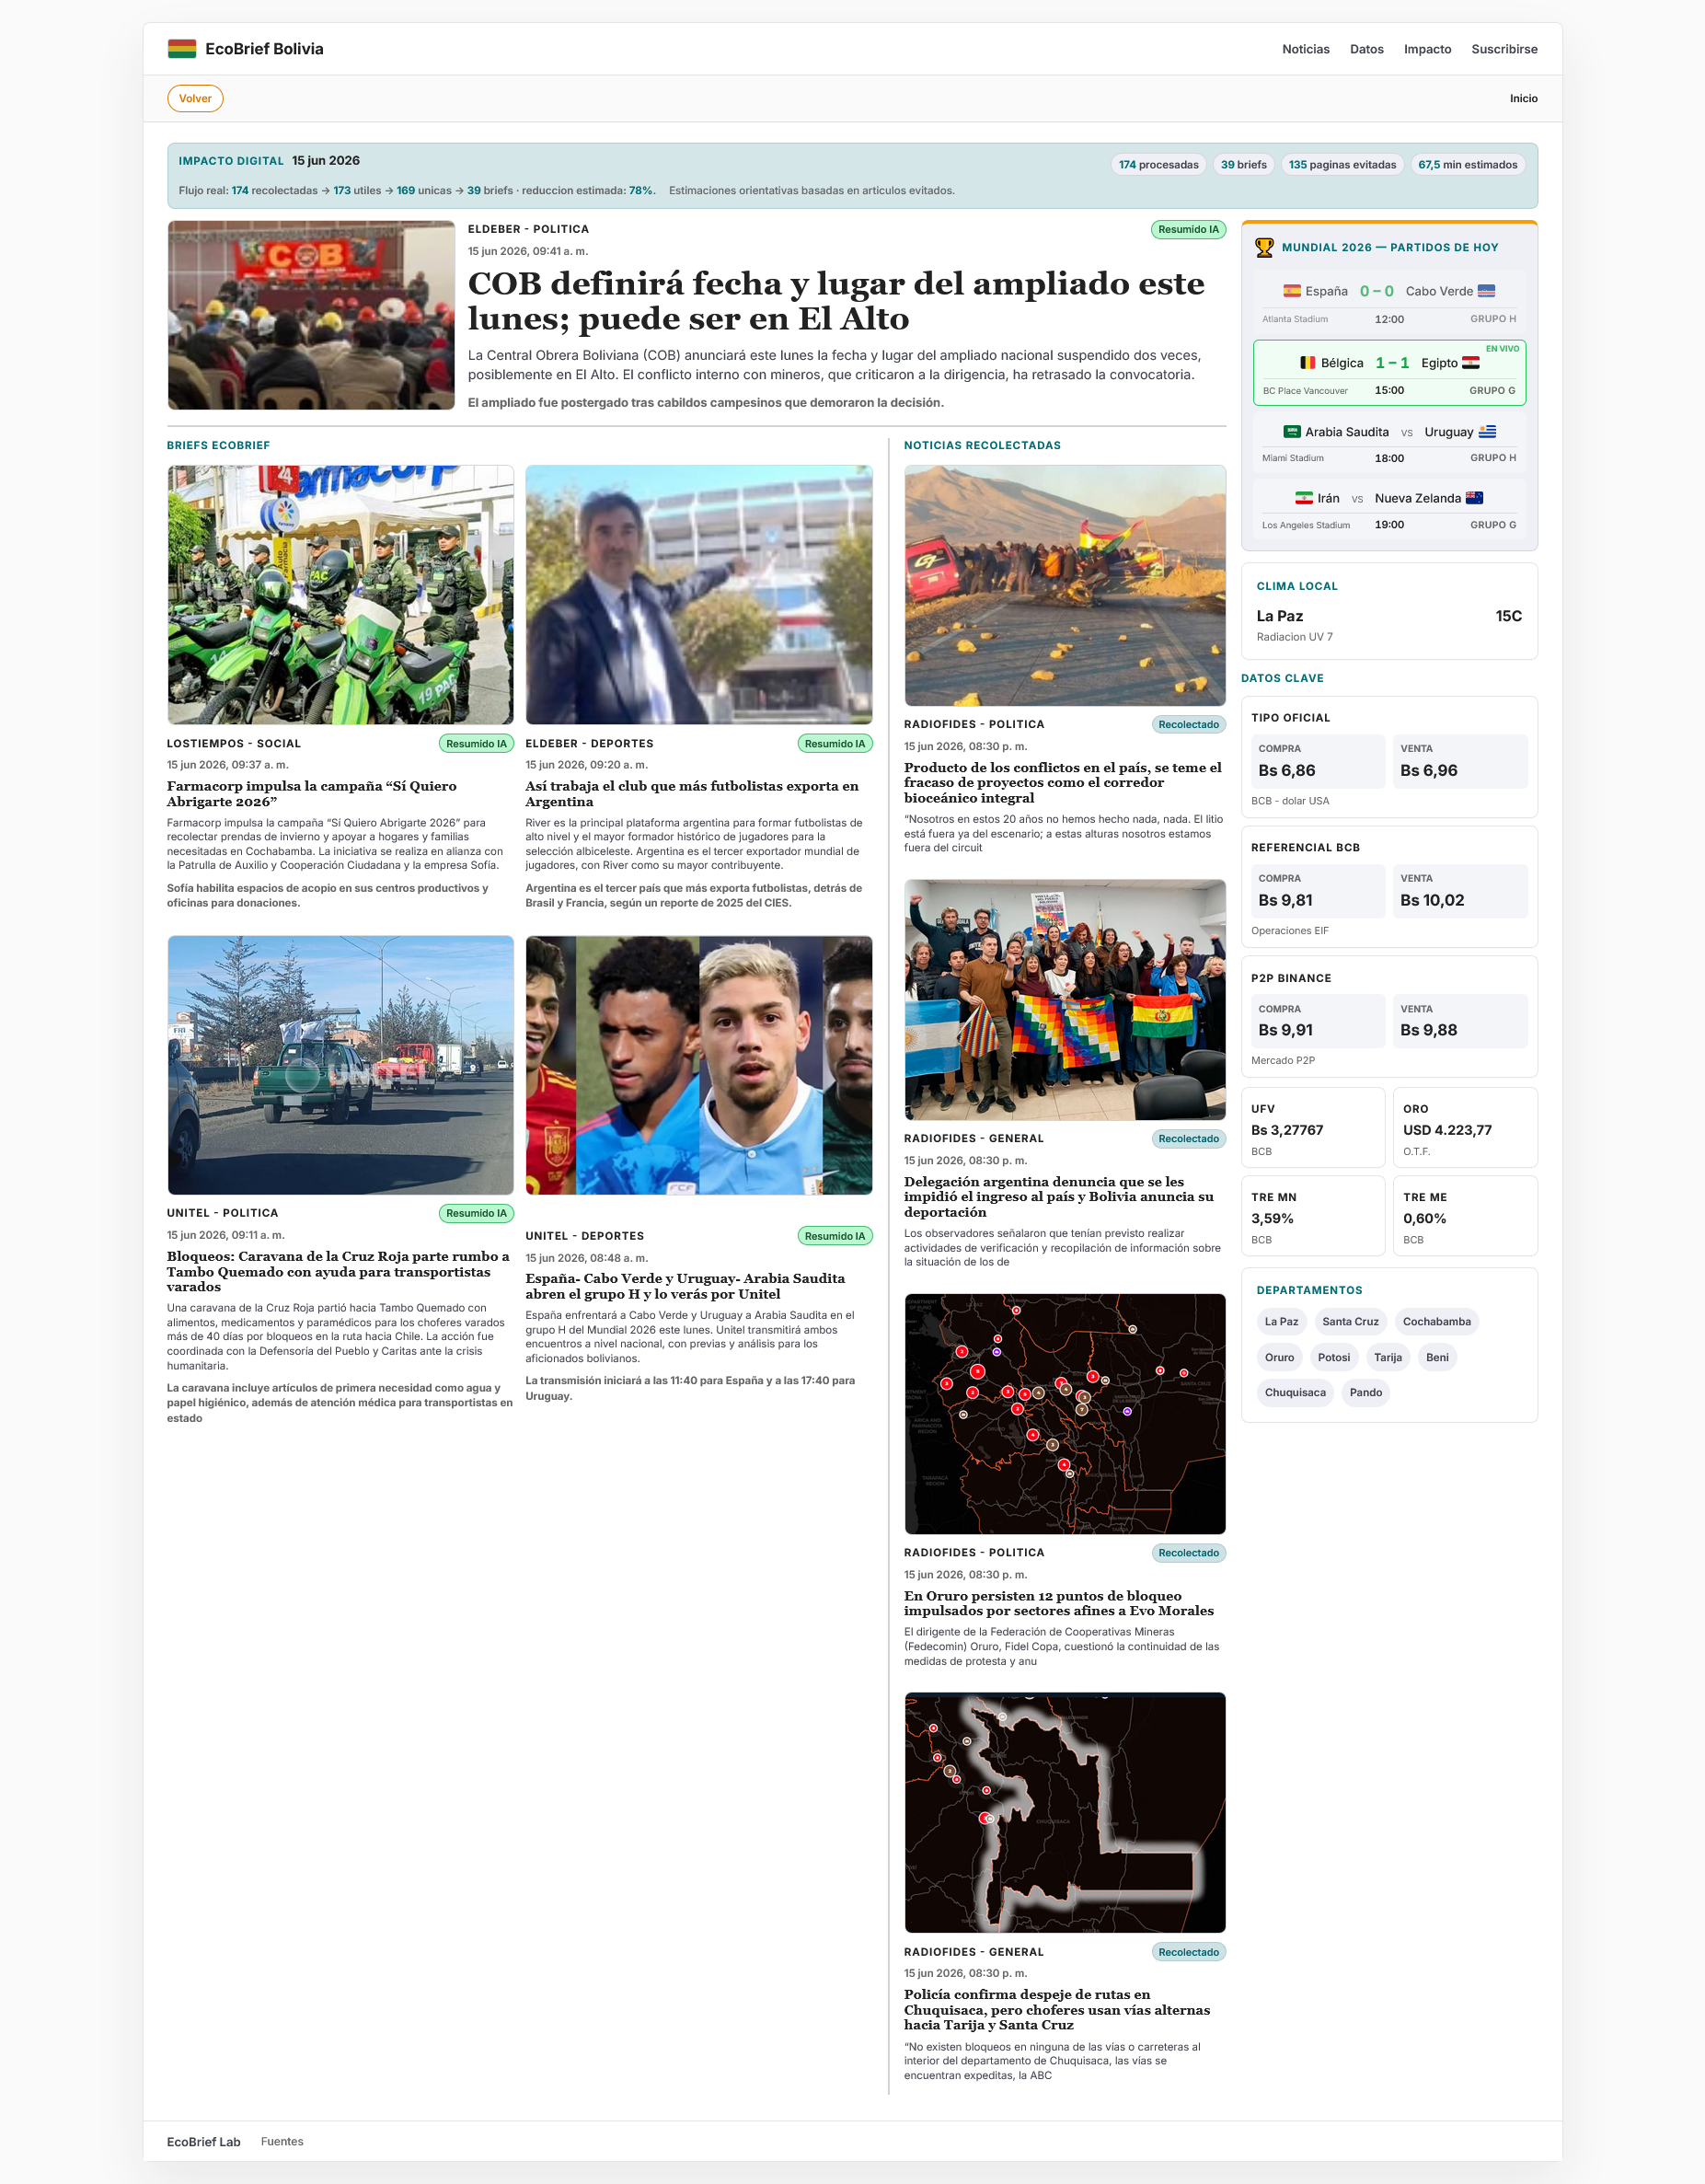
\includegraphics[width=\textwidth,keepaspectratio]{../images/1-home-page.png}
\caption{Vista principal del sistema con noticias destacadas y resumen visual}
\end{figure}

\newpage

\section*{Anexo 2: Noticias y res\'umenes}

\begin{figure}[H]
\centering
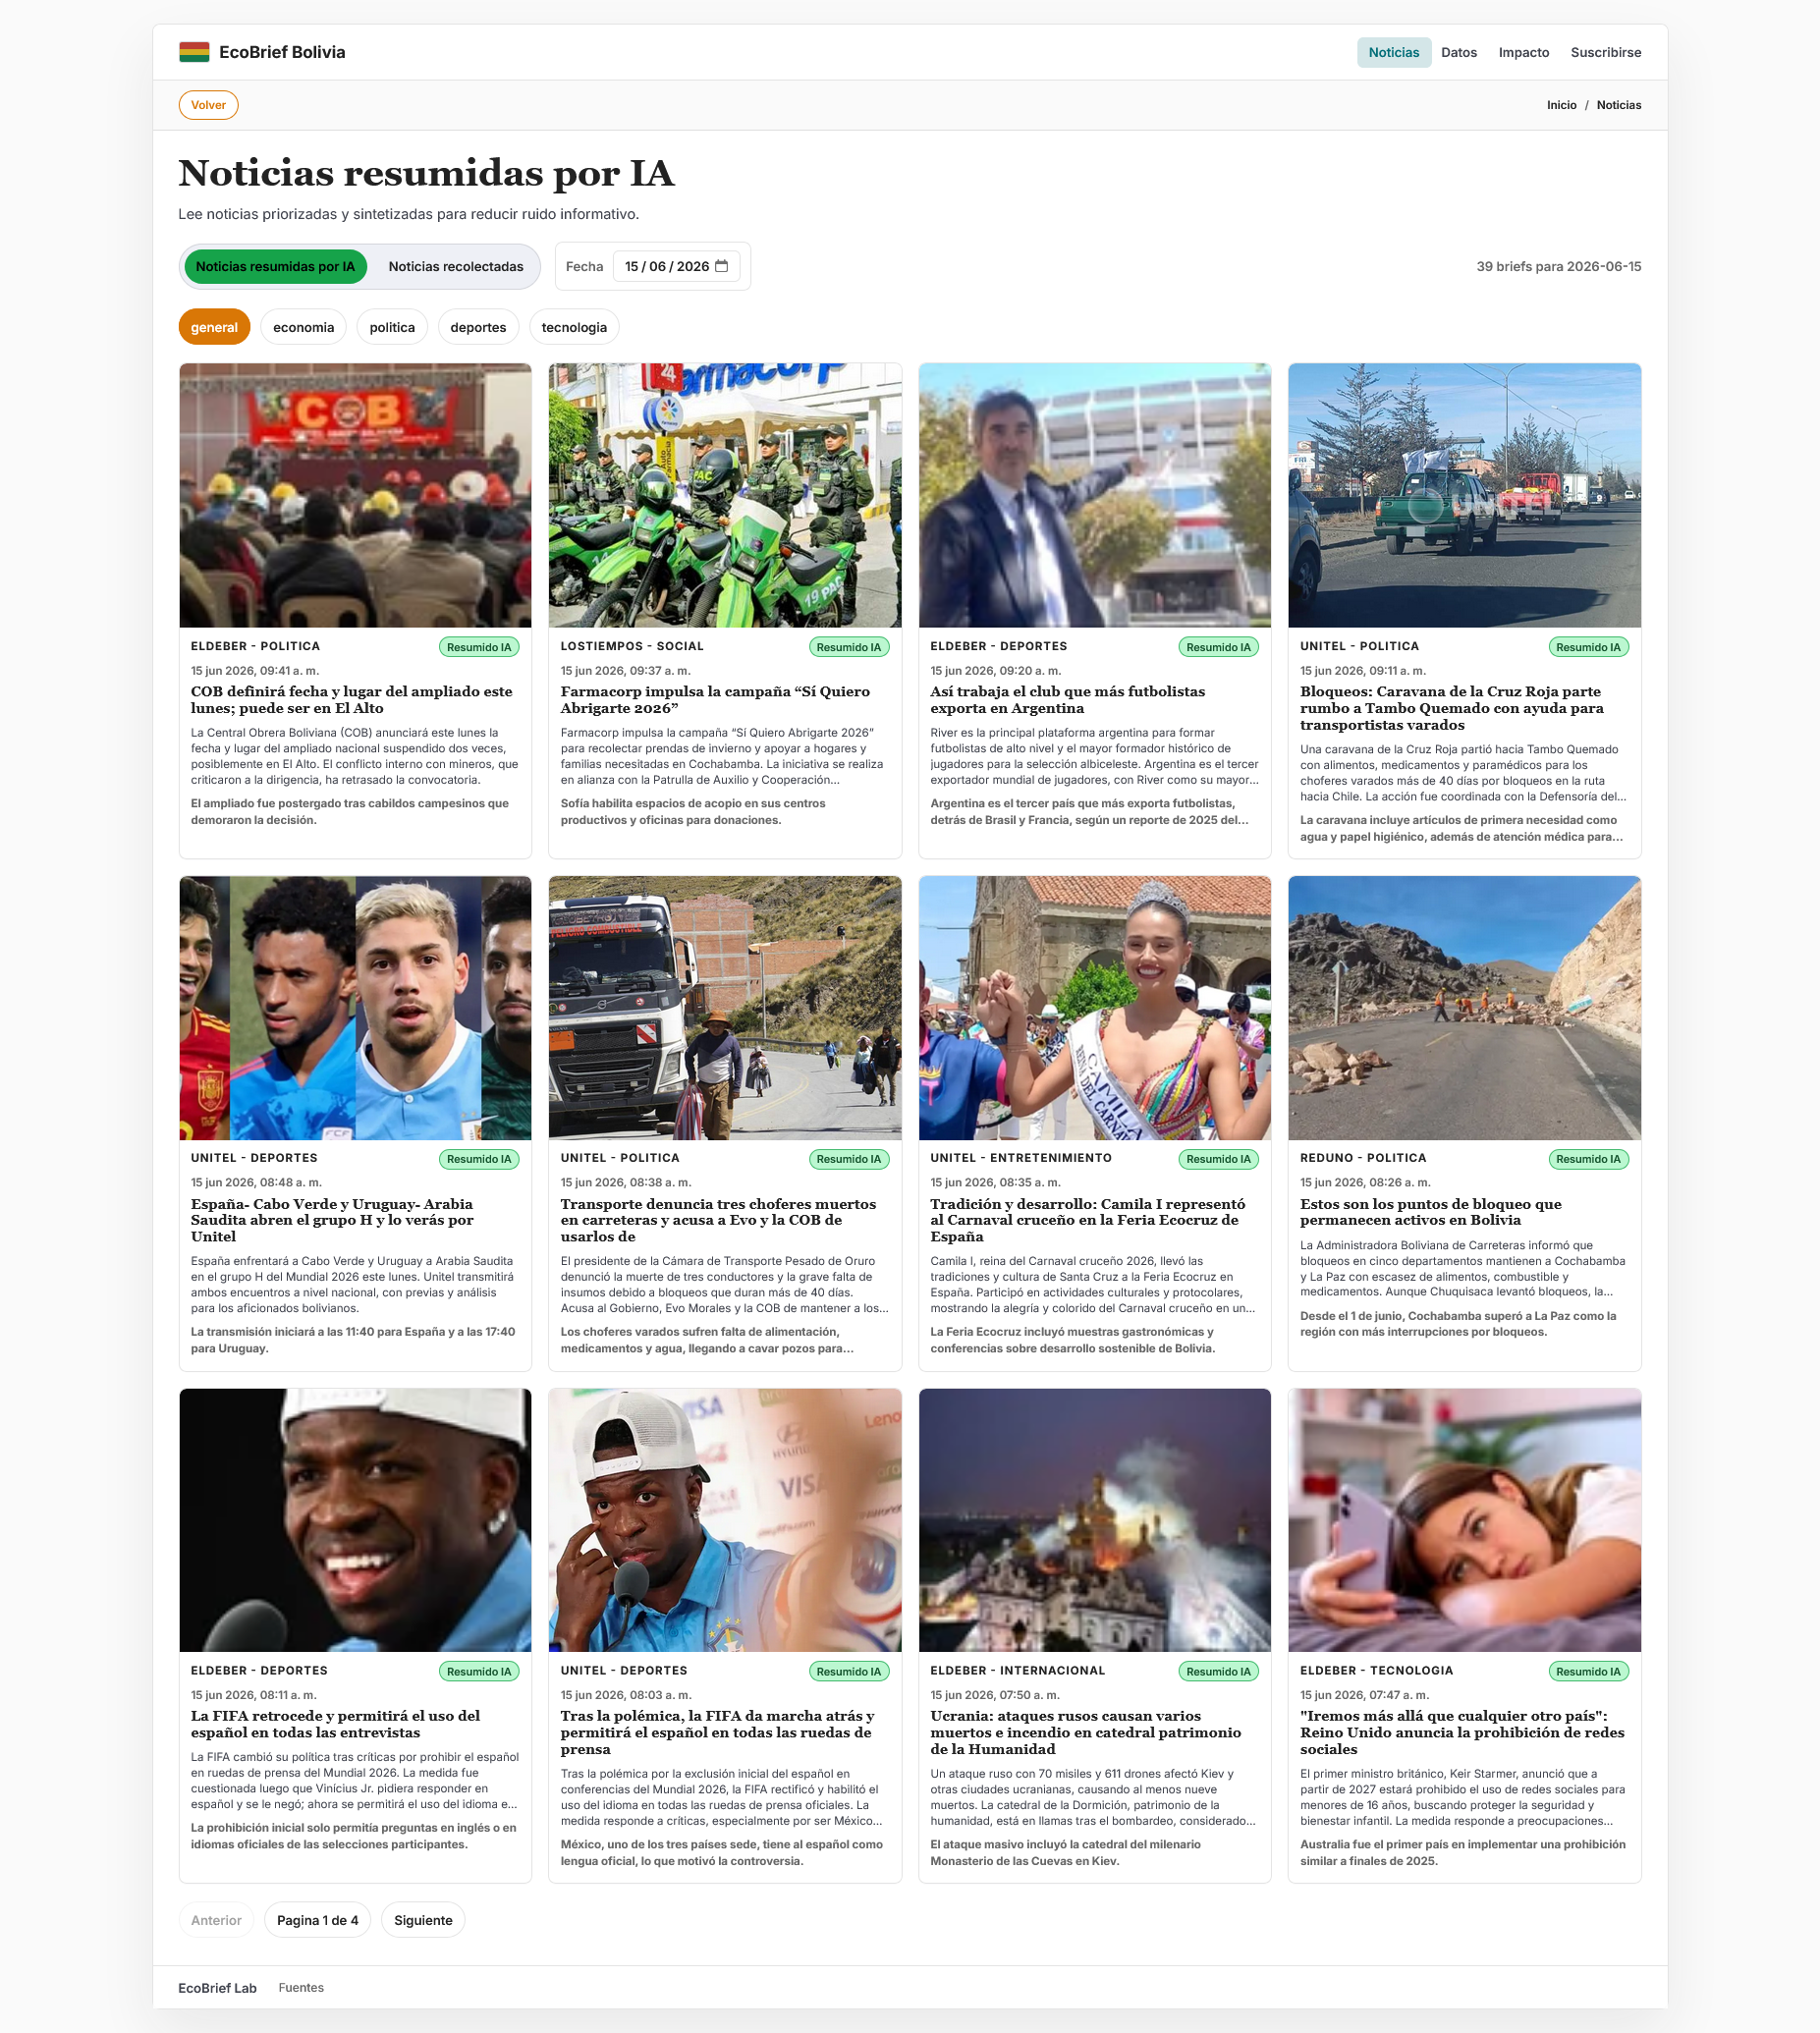
\includegraphics[width=\textwidth,keepaspectratio]{../images/2-news-summaries.png}
\caption{Listado completo de noticias con res\'umenes generados por IA}
\end{figure}

\newpage

\section*{Anexo 3: Noticias recolectadas}

\begin{figure}[H]
\centering

\includegraphics[width=\textwidth,keepaspectratio]{../images/3-news-recolectadas.png}
\caption{Panel de noticias recolectadas con detalles de fuente y fecha}
\end{figure}

\newpage

\section*{Anexo 4: P\'agina de datos}

\begin{figure}[H]
\centering
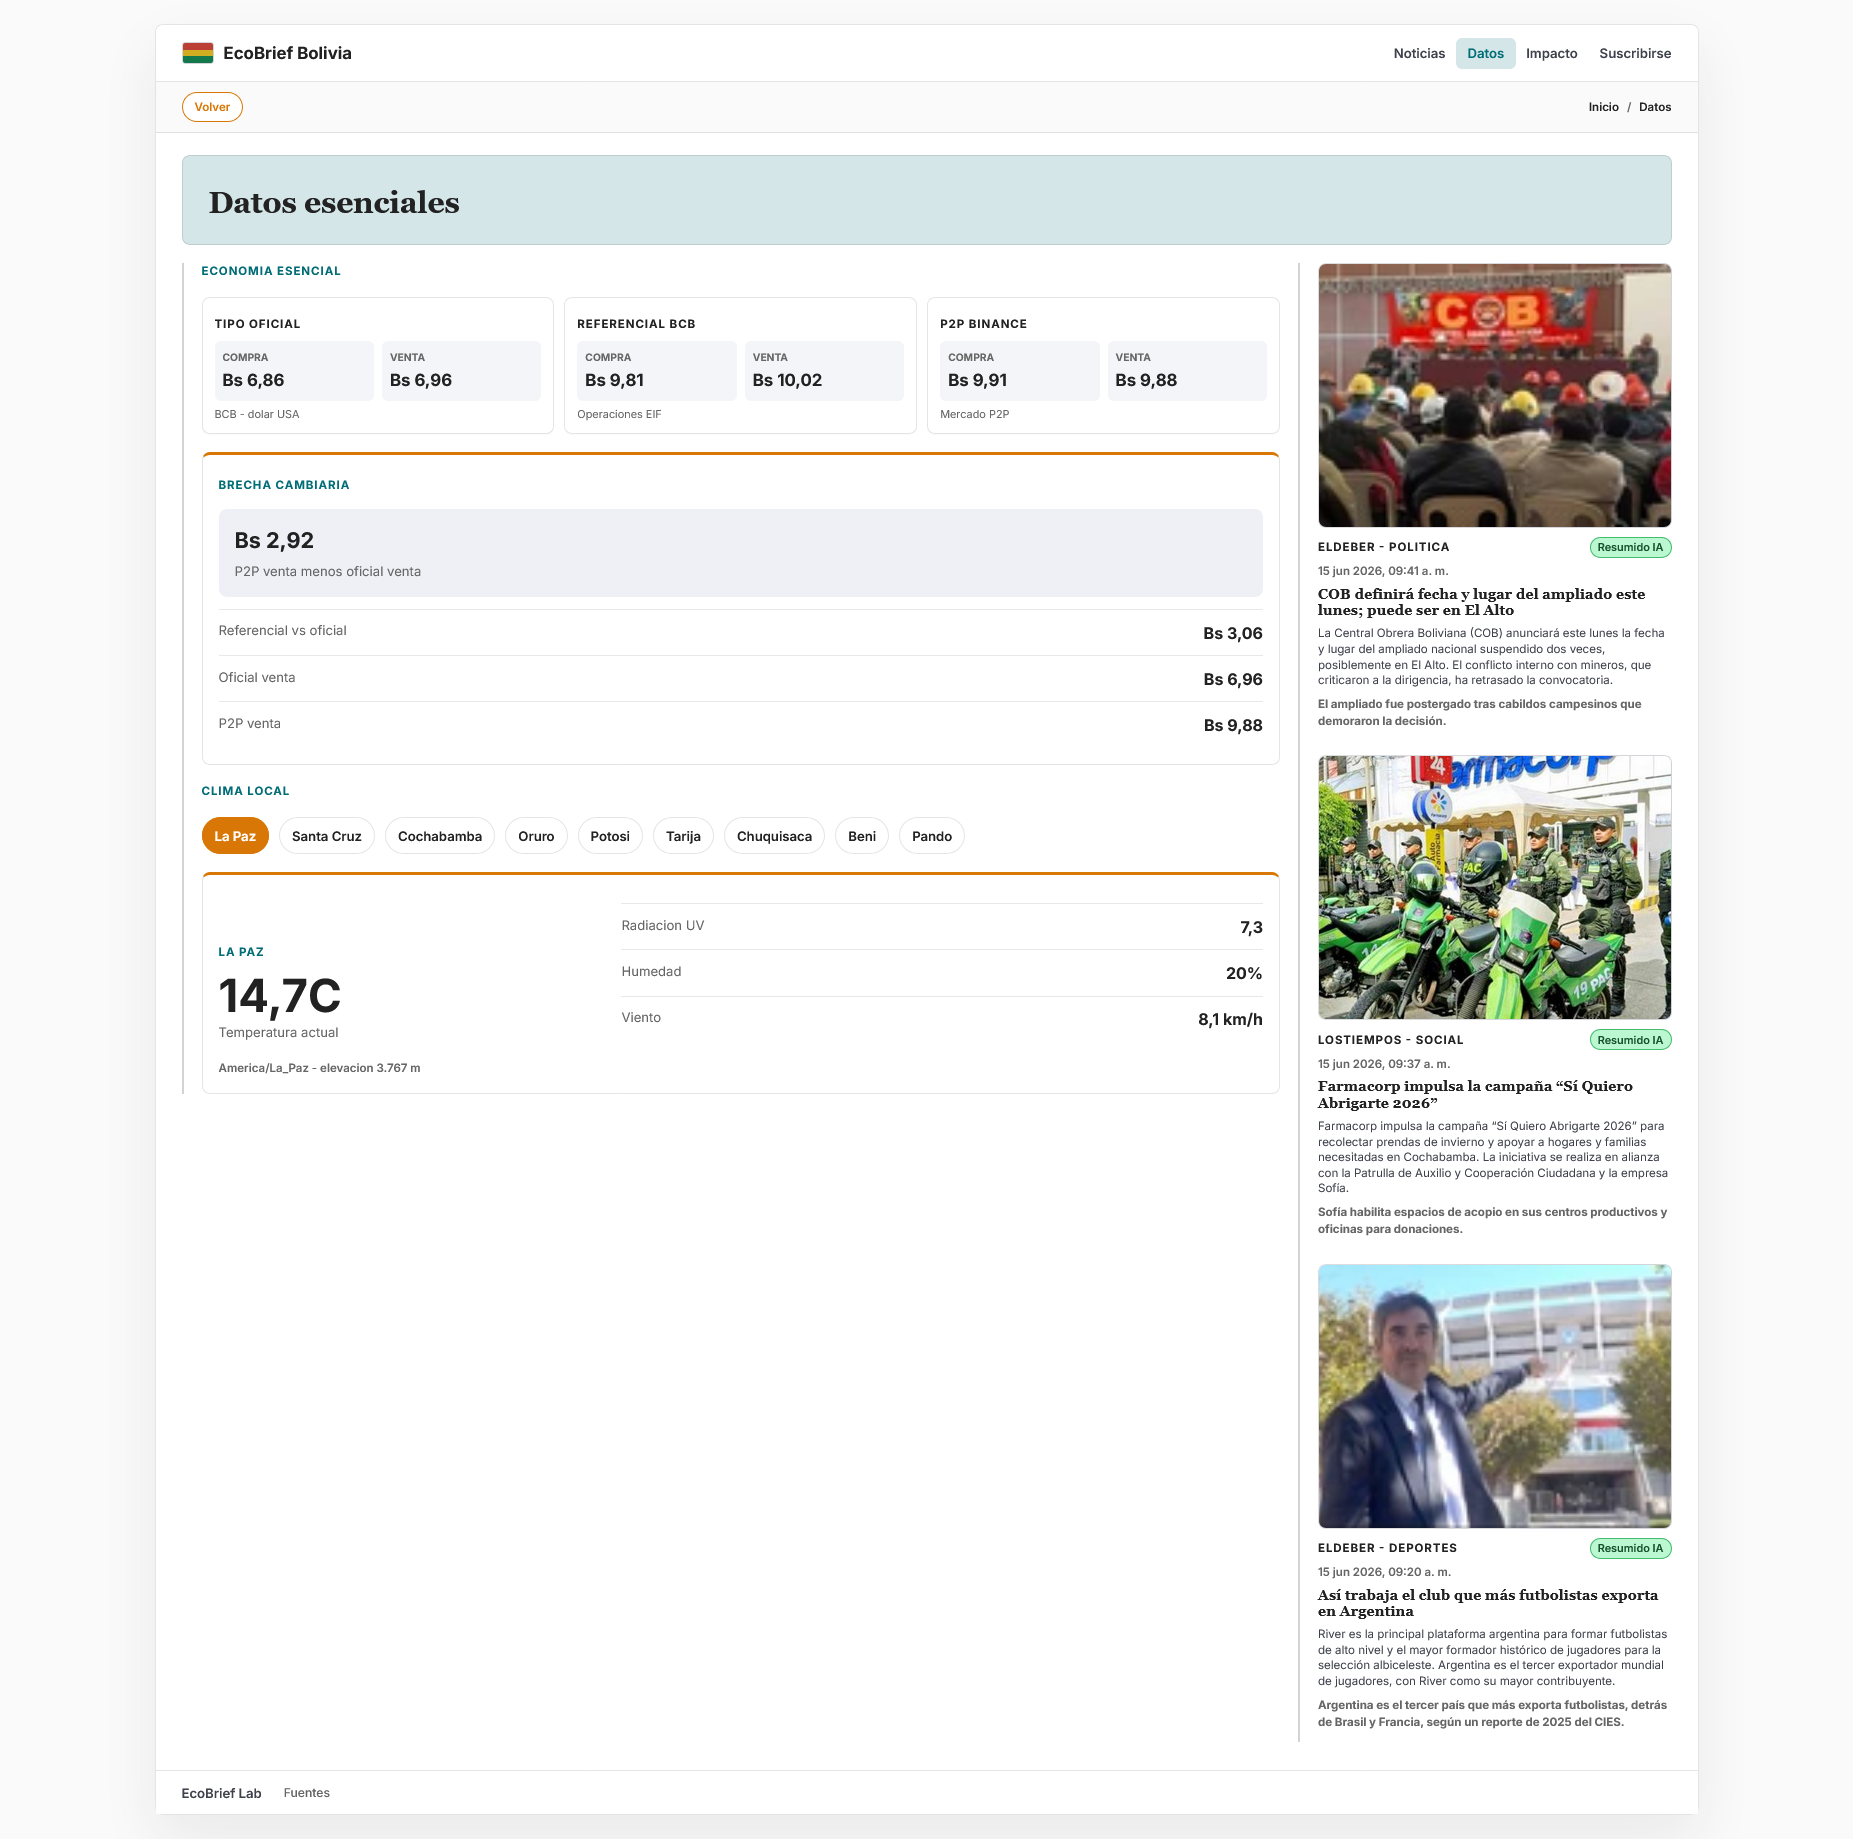
\includegraphics[width=\textwidth,keepaspectratio]{../images/4-datos-page.png}
\caption{Vista de datos e indicadores del sistema}
\end{figure}

\newpage

\section*{Anexo 5: Panel de impacto}

\begin{figure}[H]
\centering
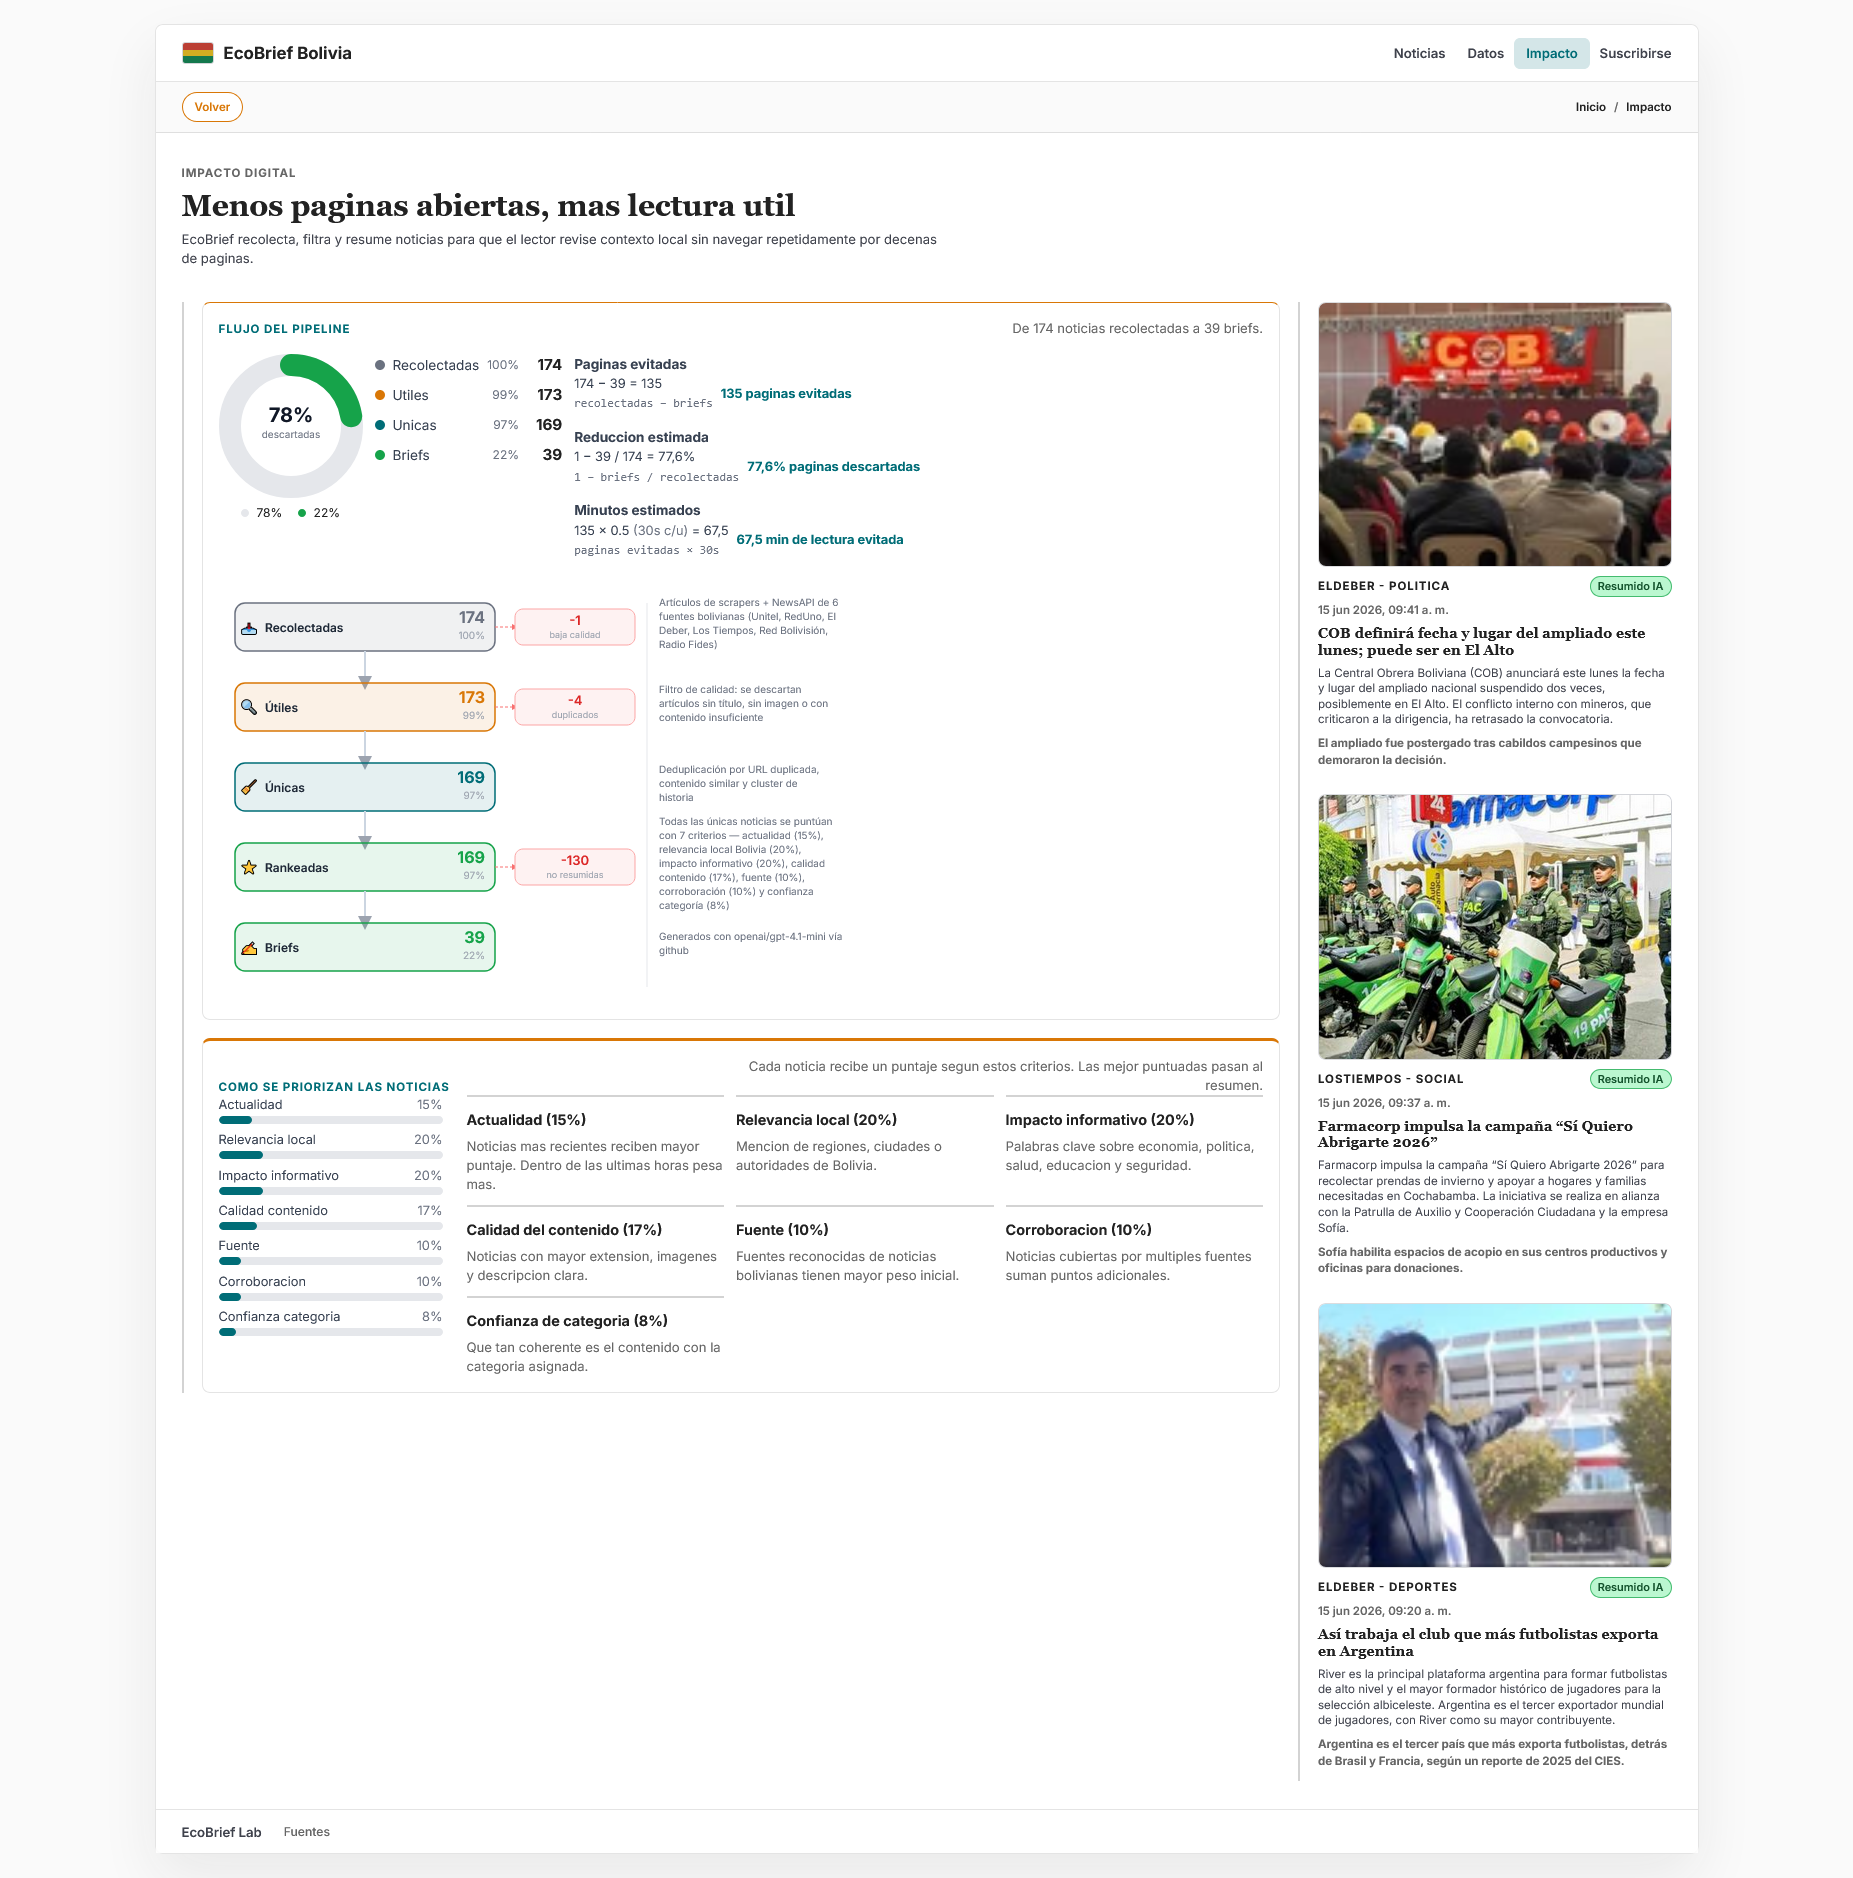
\includegraphics[width=\textwidth,keepaspectratio]{../images/5-impacto-page.png}
\caption{Panel de m\'etricas Green Tech con indicadores de impacto ambiental}
\end{figure}

\newpage

\section*{Anexo 6: Suscripci\'on y preferencias}

\begin{figure}[H]
\centering
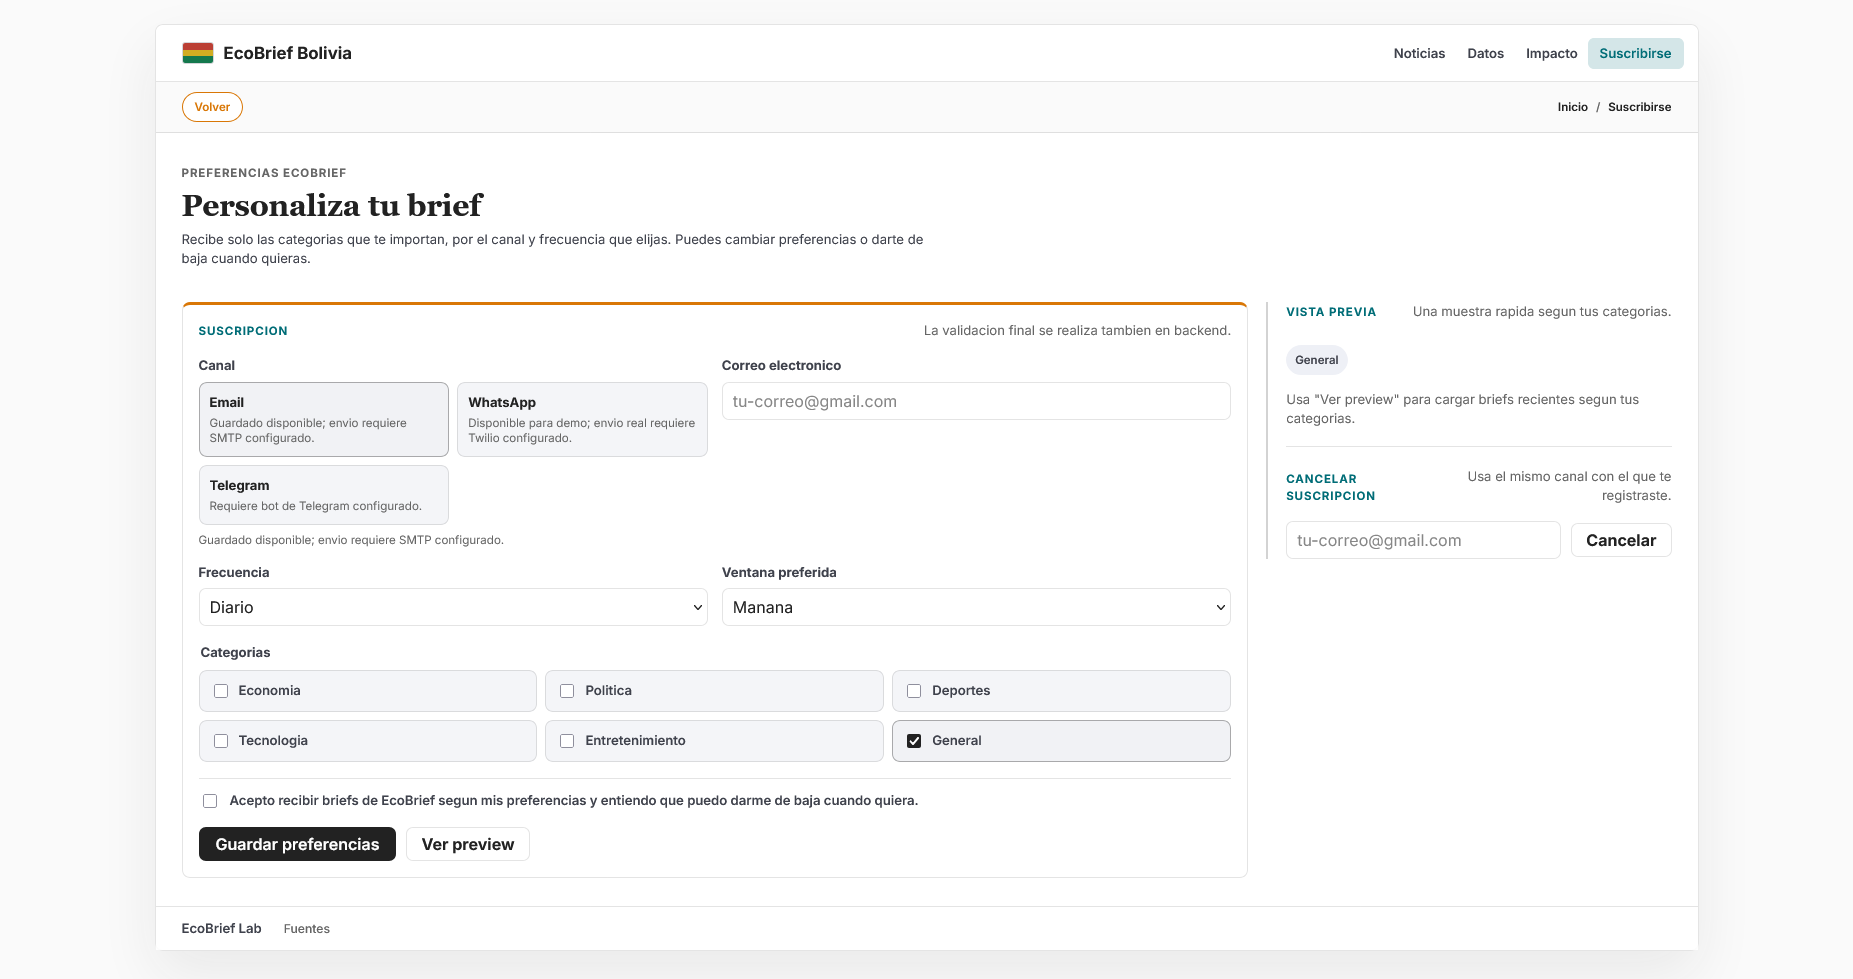
\includegraphics[width=\textwidth,keepaspectratio]{../images/6-suscripcion-page.png}
\caption{Formulario de suscripci\'on con preferencias de categor\'ia, frecuencia y canal de entrega}
\end{figure}

\chapter*{Referencias}
\addcontentsline{toc}{chapter}{Referencias}

\begin{enumerate}[nosep]
    \item Hostinger VPS KVM 2. \url{https://www.hostinger.com/vps-hosting}
    \item NIC Bolivia. Costo de dominio .bolivia.bo: 55 Bs/a\~no.
    \item Google App Passwords. \url{https://support.google.com/accounts/answer/185833}
    \item L\'imites de env\'io Gmail. \url{https://support.google.com/a/answer/166852}
    \item Twilio WhatsApp Pricing. \url{https://www.twilio.com/en-us/whatsapp/pricing}
    \item Groq Pricing. \url{https://groq.com/pricing/}
    \item DeepSeek Pricing. \url{https://api-docs.deepseek.com/quick_start/pricing}
    \item Anthropic Claude Pricing. \url{https://platform.claude.com/docs/en/about-claude/pricing}
    \item OpenAI API Pricing. \url{https://openai.com/api/pricing/}
    \item FastAPI. \url{https://fastapi.tiangolo.com/}
    \item React. \url{https://react.dev/}
    \item PostgreSQL. \url{https://www.postgresql.org/}
    \item Groq Cloud. \url{https://console.groq.com/}
    \item GitHub Models. \url{https://github.com/marketplace/models}
\end{enumerate}


\end{document}
